%!TEX root = thesis.tex

\chapter*{\vspace{-2.3cm} \Large Appendix A: Generating Suspicious Behavior \vspace{1.7cm}}
\addcontentsline{toc}{chapter}{Appendix A: Generating Suspicious Behavior}
\label{chap:pub}

\fancyhead[LO]{}
\fancyhead[RE]{Appendix B:  Generating Suspicious Behavior}

%%%%%%%%%%%%%%%%%%%%%%%%%%%%%%%%%%%%%%%%%%%

To simulate suspicious passenger behavior within ESCAPES simulator, we defined a new agent type going unnoticed from point $A$ to point $B$ as follows: suspicious agent's state contains the current position $Q_s(x,y)$. At each time step, the agent $\mathtt{s}$ computes the probability for being seen by any authority figure $\mathtt{a} \in \mathcal{S}$, where $\mathcal{S}$ is a set of authorities in a certain range. Similarly, a state of an authority agent $\mathtt{a}$ is defined by position $Q_a(x,y)$ and direction $\vec{d_a}$. Probability that the authority agents $\mathtt{a}$ sees another agent at distance $r$ with an offset angle $\theta$ from the current direction $\vec{d_a}$ is defined as a bivariate normal distribution $N_a(r, \theta)$ as shown in Figure~\ref{fig:bivariate}.

\begin{figure}[!ht]
\centering
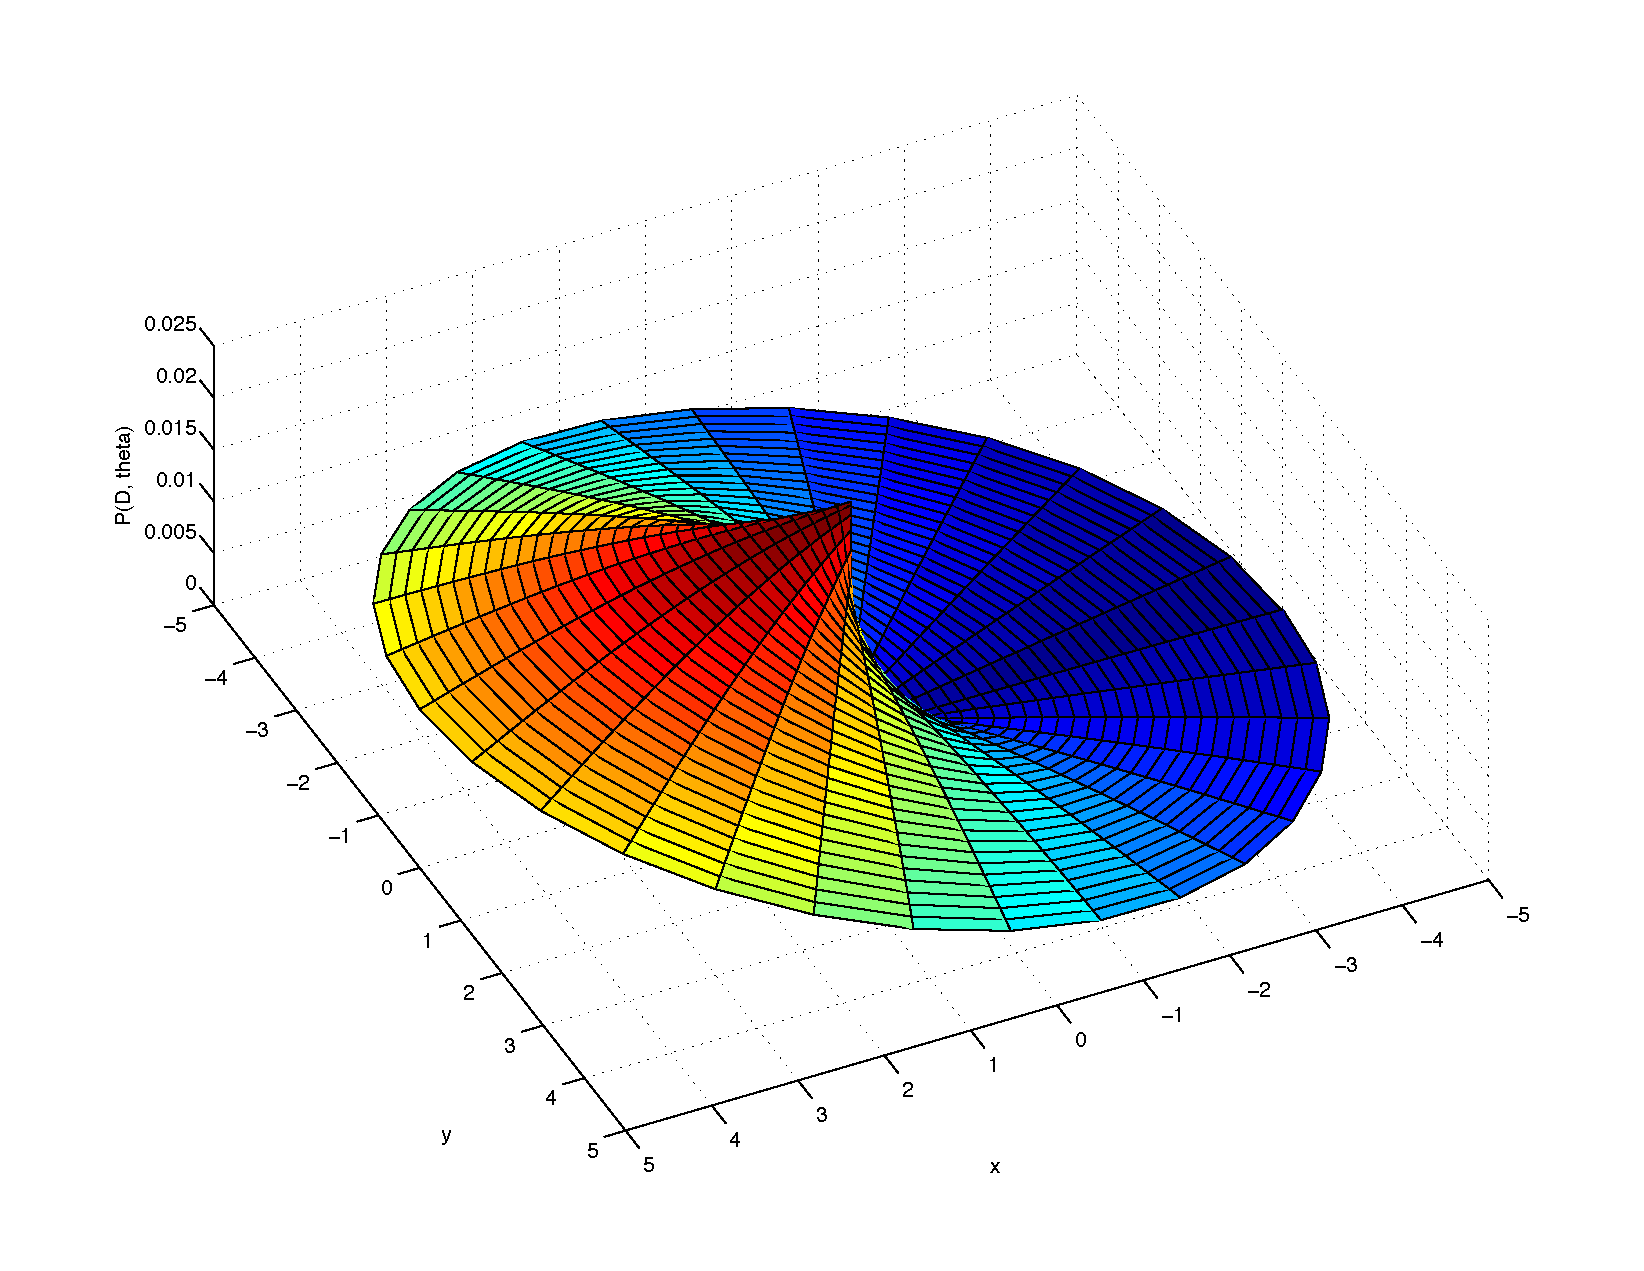
\includegraphics[width=\linewidth]{chap_surveillance/authority}
%\caption{Authority's viewpoint bounded by distance $r$ and angle $\theta$ is modeled with bivariate normal distribution $N(r, \theta)$. Warmer color represents higher and cold color represents lower probability too see a particular point.}
\caption{Authority's viewpoint modeled with bivariate normal distribution $N(r, \theta)$. Warmer color represents higher probability too see a particular point.}
\label{fig:bivariate}
\end{figure}

Points $A$ and $B$ are randomly chosen for each independent simulation. When the agent $\mathtt{s}$ reaches the point $B$, the simulation ends. The behavior of the suspicious agent follows a few simple rules:
\begin{enumerate}
 	\item Compute $p$ as a sum of probabilities for being seen by any authority figure $\mathtt{a} \in A$ in the current position $Q_s$ (and nearby $\pm\epsilon$ region)
	\begin{equation}
		p = \sum_{a \in A} \iint_{Q_s-\epsilon}^{Q_s+\epsilon}N_a(r, \theta) 
	\end{equation}
	\item If $p$ exceeds a threshold value, then compute eight random points $c_i \in C$ in radius $r$, else restore the original final point $B$ and go to step 4.
	\item Select a point such that the sum of probabilities among the current point $Q_s$ and the end point $c_i$ is the smallest 
	\begin{equation*}
		\operatorname*{arg\,min}_{c_i \in C}\sum_{a \in A}\int_{Q_s}^{c_i}N_a(r, \theta)
	\end{equation*}
	and define it as a new final point $B'$.
	\item Move towards the final point. If the distance $d(Q_s, B) < \epsilon$, end, else go to step 1.
\end{enumerate}

%Although there is a single procedure defining actions of suspicious agent, t
The resulting behavior is quite convincing and complex; ability to take into account several authorities and find the best solution in the given situation results in avoiding authorities in a half circle, making U-turns and continuing in the opposite direction, and even hiding in nearby stores. A visualization of the airport with viewpoint cones for eight authorities is shown in Figure~\ref{fig:airport:authorities}.

\begin{figure}[!ht]
\centering
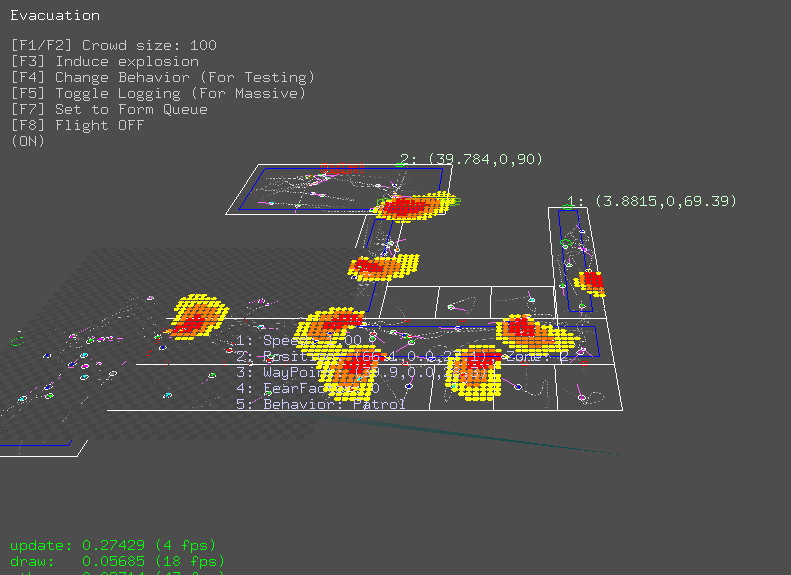
\includegraphics[width=\linewidth]{chap_surveillance/airport2}
%\caption{Authority's viewpoint bounded by distance $r$ and angle $\theta$ is modeled with bivariate normal distribution $N(r, \theta)$. Warmer color represents higher and cold color represents lower probability too see a particular point.}
\caption{Authorities' viewpoints at the airport displayed with colormap: red for high and yellow for low probability.}
\label{fig:airport:authorities}
\end{figure}